% !!! Please Don't CHANGE THESE !!! INSTEAD DEFINE YOUR OWN texdirectives.tex !!!
% These flags are for the final camera ready version for POPL
% Draft, full version flags
\newif\ifdraft\drafttrue
\newif\iffull\fullfalse
\newif\ifanon\anonfalse
\newif\iflast\lasttrue

% !!! PLEASE DON'T CHANGE THESE !!! INSTEAD DEFINE YOUR OWN texdirectives.tex !!!
\makeatletter \@input{texdirectives} \makeatother

\documentclass[acmsmall,review]{acmart}\settopmatter{}

%% Note: Authors migrating a paper from PACMPL format to traditional
%% SIGPLAN proceedings format should change 'acmlarge' to
%% 'sigplan,10pt'.


%% Some recommended packages.
\usepackage{booktabs}   %% For formal tables:
                        %% http://ctan.org/pkg/booktabs
\usepackage{subcaption} %% For complex figures with subfigures/subcaptions
                        %% http://ctan.org/pkg/subcaption

\usepackage{xspace}
\usepackage{preamble}
\usepackage{relsize}
\usepackage{float}
\usepackage{cleveref}
%\usepackage{mathpartir}

\makeatletter\if@ACM@journal\makeatother
%% Journal information (used by PACMPL format)
%% Supplied to authors by publisher for camera-ready submission
% \setcopyright{rightsretained}
% \acmJournal{PACMPL}
% \acmYear{2018} \copyrightyear{2018} \acmVolume{2} \acmNumber{POPL} \acmArticle{45} \acmMonth{1} \acmPrice{}\acmDOI{10.1145/3158133}

%% Copyright information
%% Supplied to authors (based on authors' rights management selection;
%% see authors.acm.org) by publisher for camera-ready submission
%\setcopyright{acmcopyright}
%\setcopyright{acmlicensed}
%\setcopyright{rightsretained}
%\copyrightyear{2017}           %% If different from \acmYear


%% Bibliography style
\bibliographystyle{ACM-Reference-Format}
%% Citation style
%% Note: author/year citations are required for papers published as an
%% issue of PACMPL.
\citestyle{acmauthoryear}   %% For author/year citations

\def\l{l}

\begin{document}

%% Title information
\title{Keep your Laziness in Check}
                                        %% when present, will be used in
                                        %% header instead of Full Title.
%\titlenote{with title note}             %% \titlenote is optional;
%                                        %% can be repeated if necessary;
%                                        %% contents suppressed with 'anonymous'
%\subtitle{}                     %% \subtitle is optional
%\subtitlenote{with subtitle note}       %% \subtitlenote is optional;
                                        %% can be repeated if necessary;
                                        %% contents suppressed with 'anonymous'


%% Author information
%% Contents and number of authors suppressed with 'anonymous'.
%% Each author should be introduced by \author, followed by
%% \authornote (optional), \orcid (optional), \affiliation, and
%% \email.
%% An author may have multiple affiliations and/or emails; repeat the
%% appropriate command.
%% Many elements are not rendered, but should be provided for metadata
%% extraction tools.

%% Author with single affiliation.
\author{Kenneth Foner}
%\authornote{with author1 note}          %% \authornote is optional;
                                        %% can be repeated if necessary
%\orcid{nnnn-nnnn-nnnn-nnnn}             %% \orcid is optional
\affiliation{
%  \position{Position1}
%  \department{Department1}              %% \department is recommended
  \institution{University of Pennsylvania}            %% \institution is required
%  \streetaddress{Street1 Address1}
%  \city{City1}
%  \state{State1}
%  \postcode{Post-Code1}
  \country{USA}
}
\email{kfoner@seas.upenn.edu}          %% \email is recommended

%% Author with single affiliation.
\author{Hengchu Zhang}
%\authornote{with author1 note}          %% \authornote is optional;
                                        %% can be repeated if necessary
%\orcid{nnnn-nnnn-nnnn-nnnn}             %% \orcid is optional
\affiliation{
%  \position{Position1}
%  \department{Department1}              %% \department is recommended
  \institution{University of Pennsylvania}            %% \institution is required
%  \streetaddress{Street1 Address1}
%  \city{City1}
%  \state{State1}
%  \postcode{Post-Code1}
  \country{USA}
}
\email{hengchu@seas.upenn.edu}          %% \email is recommended

%% Author with single affiliation.
\author{Leonidas Lampropoulos}
%\authornote{with author1 note}          %% \authornote is optional;
                                        %% can be repeated if necessary
%\orcid{nnnn-nnnn-nnnn-nnnn}             %% \orcid is optional
\affiliation{
%  \position{Position1}
%  \department{Department1}              %% \department is recommended
  \institution{University of Pennsylvania}            %% \institution is required
%  \streetaddress{Street1 Address1}
%  \city{City1}
%  \state{State1}
%  \postcode{Post-Code1}
  \country{USA}
}
\email{llamp@seas.upenn.edu}          %% \email is recommended

%% Paper note
%% The \thanks command may be used to create a "paper note" ---
%% similar to a title note or an author note, but not explicitly
%% associated with a particular element.  It will appear immediately
%% above the permission/copyright statement.
%\thanks{with paper note}                %% \thanks is optional
                                        %% can be repeated if necesary
                                        %% contents suppressed with 'anonymous'


%% Abstract
%% Note: \begin{abstract}...\end{abstract} environment must come
%% before \maketitle command
\begin{abstract}
StrictCheck.

Because LazyCheck was taken.
\end{abstract}


%% 2012 ACM Computing Classification System (CSS) concepts
%% Generate at 'http://dl.acm.org/ccs/ccs.cfm'.
\begin{CCSXML}
<ccs2012>
<concept>
<concept_id>10011007.10011006.10011008</concept_id>
<concept_desc>Software and its engineering~General programming languages</concept_desc>
<concept_significance>500</concept_significance>
</concept>
</ccs2012>
\end{CCSXML}

\ccsdesc[500]{Software and its engineering~General programming languages}
%% End of generated code


%% Keywords
%% comma separated list
\keywords{Random Testing, Laziness, Haskell}  %% \keywords is optional

%% \maketitle
%% Note: \maketitle command must come after title commands, author
%% commands, abstract environment, Computing Classification System
%% environment and commands, and keywords command.
\maketitle

% \lk{
% \begin{description}
%   \item[slant] \the\fontdimen1\font
%   \item[interword space] \the\fontdimen2\font
%   \item[interword stretch] \the\fontdimen3\font
%   \item[interword shrink] \the\fontdimen4\font
%   \item[extra space] \the\fontdimen7\font
%   \item[xspaceskip] \the\xspaceskip
%   \item[hyphenchar] \the\hyphenchar\font
% \end{description}
% }

\section{Introduction}
\label{sec:intro}

%\hzh{Rewrite the intro using different running examples, foldl vs foldr on stream manipulations?}
%\hzh{We can write a hand-crafted spec for take, can we show that we can create this spec by composing the spec for foldr (but not using the one with foldl)}
%\hzh{implement take in 3 ways: foldl, foldr and explicitly as the opening example, and then ask if they're equivalent? (they're not!)}
\hzh{Okasaki has 2 functions that appends a list to the reversal of another list, one of which is too strict and the other one is just the right amount of lazy (thus incremental)}
\hzh{The amortized one is hard to specify exactly, but we can introduce approximate specification and specify it approximately}
\hzh{we need to carefully avoid saying this is a tool for specifying the time complexity of functions}
\hzh{Implementing functional programs that make clever use of laziness is very easy to get wrong, and we provide a solution to make sure the programmer got it right. We almost have no way of testing it right now before StrictCheck.}
\hzh{Email Ryan Trinkle and Dan Winograd-Cort about FRP and strictness, and try to use their examples as another problem we can solve in the intro}
\hzh{Maps will mess up memoization if you're overly strict, use knapsack as an example}

\leo{Point of first paragraph: lazy evaluation is powerful}
\caleb{What does the word ``power'' mean? It's non-specific. Useful? Convenient?}

Lazy evaluation gives tremendous power to functional programmers
~\cite{WhyFPMatters} and is actively used in various practical
applications. For instance, the big-data framework Spark uses laziness
to drive computations on demand\cn, Apple's programming language Swift
leverages it to initialize expensive resources as needed\cn, and many
functional reactive programming web frameworks rely on
it crucially\cn \leo{This point might need more exposition about frp}. Haskell
is the most popular programming language that allows programmers to
enjoy the power of lazy evaluation by default. However, it
does not come without a price.
\leo{Didn't we have an FRP quote by someone that Laziness was the third source of
bugs or something? Work that in?}
\hzh{Ryan Trinkle (author of Reflex) said laziness was the 3rd most difficult thing to
get right, but let's check with him on whether we can quote him on that.}

\caleb{Again, power and responsibility are not completely clear, but I do like the narrative}
The power of laziness puts great responsibility on programmers'
shoulders. An implementation that uses laziness incorrectly can either
behave functionally the same but with inferior \caleb{Inferior than
what?} performance---compared to a strict counterpart, or it can
completely break down!\caleb{unclear. loops?} Reasoning about lazy
programs is also notoriously hard --- the programmer needs to have a
mental model of the order of evaluation of the code, and this order is
not always obvious from the syntax of the code.

How, then, can we test and catch such laziness bugs during
development? Is it possible to precisely specify laziness behavior
just as we would for functional correctness?
%
In this paper, we demonstrate techniques for observing laziness in
Haskell, and propose a system of creating specifications of lazy
Haskell programs. We implement these ideas as a Haskell library. For
concreteness, consider the following example using the standard
\lk{take} function on lists, which accepts an integer $n$ and a list, and returns
a prefix of the list with length $n$. If $n$ is larger than the length
of the original list, then the entire list is returned.
%
\begin{inlinecode}
take_spec :: Shaped a => Spec '[Int, [a]] [a]
take_spec =
  Spec $ \predict d n xs ->
    predict n (if n > length xs then d else d ++ thunk)
\end{inlinecode}
%
The \lk{Spec} constructor takes a function, whose first
argument \lk{predict} is the predicted demand on the \lk{Int} argument
of \lk{take}, and second argument the predicted demand on the \lk{[a]}
argument. This spec simply says that the \lk{Int} argument will always
be used, and the demand on the list argument is either the same as the
demand on the output, or demand on the output plus some
unevaluated \lk{thunk} at the end. The former case happens when $n$ is
larger than the list's length, otherwise the latter case applies.

In the next section we work through two more examples, functional
queues and functional maps, demonstrating both the difficulties of
programming with laziness and how our approach can be used to
alleviate them.
%
In the rest of the paper, we present our technical contributions:
\begin{itemize}
\item We introduce a novel approach to specifying the laziness behavior
of functions that is {\em precise} and {\em compositional}. Such
specifications are expressive enough to capture exactly how much
evaluation occurs within a data structure
%\leo{Also add
%drawbacks/partiality here? If not here, where in the intro?} \hzh{I'm
%not sure if we should bring in partiality (in the sense of
%divergence/nontermination) yet since that seems like a rather
%technical detail of the spec}
\item We propose a framework for automated testing against such specifications.\caleb{Automated testing? Can be more specific}\leo{Should we mention QuickCheck here?}
\item We improve upon the random function generators from QuickCheck\cn to generate functions with arbitrary laziness behaviors.
\item We discuss our generic programming-based impementation to apply StrictCheck to all algebraic data types.\leo{I guess ``packed'' maps do not qualified as algebraic?}
\end{itemize}
%
Section~\ref{sec:related} discusses related work. We conclude and draw
directions for future work in Section~\ref{sec:concl}.

\section{Strictness Specifications, by Example}
\label{sec:examples}

\subsection{Purely functional queues}
\label{sec:queues}

For our first example, we turn to a very popular data structure:
purely functional queues.  Such queues are typically implemented with
two lists---a front list holding the queue elements in FIFO order, and
a back list holding the other elments in reversed order. When the
front list is empty, a dequeue operation must reverse the back list to
refill the front list. These specific dequeue operations take $O(n)$
time to finish and are much slower than their imperative
counterparts, a performance degradation only compounded by
persistence---where the $O(n)$ operation could be repeated many times,
and unacceptable for many real-time systems.

Amongst his work on purely functional data structures\cite{Okasaki},
Okasaki cleverly improved upon this design using lazy lists that both
incrementally performs the reversal of the back list, and
incrementally appends the reversal of the back list onto the front
list ~\cite{Okasaki95simpleand}. Okasaki's queue relies on the
following \lk{rotate} function to incrementally reverse and append the
back list.
\begin{inlinecode}
  rotate :: [a] -> [a] -> [a] -> [a]
  rotate      []       []  as =                       as
  rotate      []  (b : bs) as =     rotate [] bs (b : as)
  rotate (f : fs)      []  as = f : rotate fs []      as
  rotate (f : fs) (b : bs) as = f : rotate fs bs (b : as)
\end{inlinecode}
If we computed the expression \lk{rotate front back []}, its value
will be equivalent to \lk{front ++ (reverse back)}. However, unlike
the naive reverse-and-append operation, \lk{rotate} is much
lazier. A \lk{reverse} function has to evaluate the entire structure
of the back list, which is not incremental. On the other
hand, \lk{rotate} produces a list immediately, and packs the rest of
the computation into the lazy list \lk{rest}.

Since \lk{rotate} is functionally equivalent to \lk{front ++ (reverse
back)}, a programmer could have implemented it naively and never
discover the mistake through traditional testing! The two only differ
in their laziness behavior. Fortunately, we can use StrictCheck to
write a specification that makes this property of \lk{rotate}
testable.

To describe the laziness behavior, we need to first introduce a few
types that describe how lists are used. We use the
term \textit{demand} to refer to the shape of such usage. Concretely,
a \textit{demand} is a shape that describes the used part of a data
structure. For lists, \textit{demands} will be prefixes of lists. We
use the type \lk{ListD} to represent such demands.
%
\begin{inlinecode}
  data ListD a = NilD
               | ConsD (Thunk a) (Thunk (ListD a))
\end{inlinecode}
%
The \lk{Thunk} type used in \lk{ListD} has 2 constructors: \lk{E}
for \textit{evaluated} and \lk{T}, a nullary constructor,
for \textit{thunk}. In \lk{ListD}, \lk{Thunk} wraps around all the
list constructor fields, and this allows us to represent lack of
further evaluation by using the \lk{T} constructor. For example, given
the list \lk{[1, 2, 3]}, the value \lk{ConsD T (ConsD T T)} represents
the \textit{demand} that reveals the first 2 \lk{Cons} constructors of
the list, but does not evaluate any other parts of the list. To
improve readability of demand values, we will also use the
syntax \lk{\_ : \_ : \_} instead of explicit demand type values. In
this expression, the first two underscores represent unevaluated
elements in the list, while the last underscore represents unevaluated
tail of the list.

In Haskell, to trigger the evaluation of a lazy function, we need to
exert some demand on the result of that function. This suggests a
natural flow for the specification of a lazy function --- given the
demand on the output, the specification should calculate the demands
on the input. However, this is not enough in general because the
demand on the input could depend on the \textit{value} of the inputs
as well. The \lk{take} function introduced in \Cref{sec:intro} is such
a case.

Putting these pieces together, we can specify the laziness behavior
of \lk{rotate} with Okasaki's insight: as long as the front list is
longer than the back list, demanding the first element from the result
of \lk{rotate} only causes evaluation of the first element of the
front list ~\cite{Okasaki95simpleand}. Since \lk{rotate} is always
used by supplying the empty list \lk{[]} as the accumulator argument,
we define \lk{rot fs bs = rotate fs bs []}, and show a specification
of \lk{rot}.
%
\begin{inlinecode}
rot_spec :: Shaped a => Spec '[[a], [a]] [a]
rot_spec =
  Spec $ \predict d fs bs ->
    let (fs', bs') = splitAt (length fs) (cap d)
        spineLen  = length (cap (d ++ [undefined]))  -- # of spine thunks forced
        overflow  = spineLen       > length fs  -- begun taking from bs?
        overrot   = length (cap d) > length bs  -- forced all of bs?
        padLength =
          length bs `min`
            if overflow
            then length bs - length bs'
            else length (cap d)
        spinePad = replicate padLength thunk
    in predict
         (                    fs' ++ if overflow            then [] else thunk)
         (spinePad ++ reverse bs' ++ if overflow || overrot then [] else thunk)
\end{inlinecode}
%
The \lk{rotate\_spec} exactly captures the core idea from Okasaki's \lk{rotate}
operation, and testing the reverse and append implementation against this
specification immediately produces a counter example.
\begin{figure}[H]
\centering
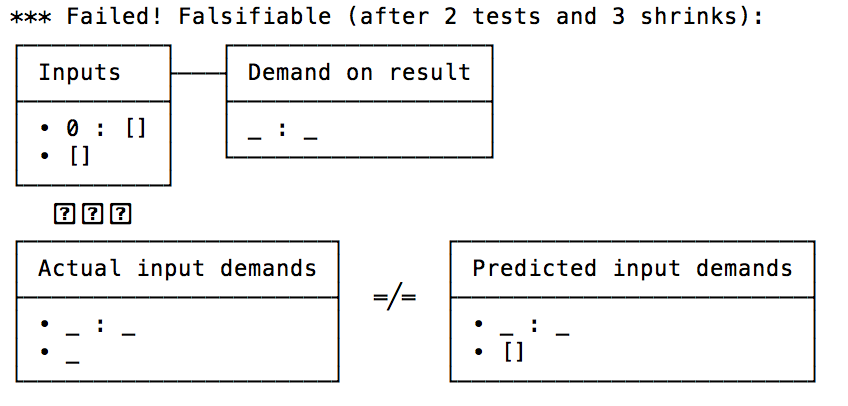
\includegraphics[width=0.8\textwidth]{revappend_counterexample}
\caption{Counterexample for \lk{revAppend} under \lk{rot\_spec}}
\end{figure}

\subsection{Key- vs value-strict maps}

\leo{Example 2: Maps / Knapsack}

For the second example, we turn to a different functional data structure where
both a strict and a lazy variant can be situationally useful: maps. There are
two reasonable laziness behaviors that implement a map interface; we could
implement a completely strict map, or we could lazily evaluate the values stored
as needed.
\footnote{A third option could be to have lazy keys, but they would
necessarily be forced at every insertion or lookup, with no gain.}
Haskell's standard library provides these two variants in the form of
\lk{Data.Map.Strict} and \lk{Data.Map.Lazy}. However, there is no way
to {\em specify} the difference between the two versions! At best, one
could hope for a hand-crafted suite of unit tests containing divergent
terms to observe a difference in termination.
\leo{One thing we could do is ignore the knapsack and expand on the above.}
\leo{Here we need a similar discussion as with lists}


Moreover, it is important to be able to distinguish whether such a datatype
follows a desired laziness behavior. For instance, the standard functional
solution for dynamic programming problems crucially uses laziness \hzh{is this
solution really standard? Is there some work we can cite to establish this
approach as the canonical approach for dynamic programming in functional
programming?}. Let us consider the famous knapsack problem.
%
The inputs of the problem are two sequences of numbers $w_i$ and $v_i$
where $i = 1, \dots, n$, and each of $w_i$ and $v_i$ specify the
weight and the value of the $i$th item. The solution presents the
maximum value achievable using a subset of the items such that their
combined weight is under a limit $W$.
%
The usual dynamic programming approach for knapsack maintains a
table $OPT[][]$, where the entry $OPT[j][k]$ keeps the best value
achievable using only items $1\dots j$ and a weight limit of $k$. The
table satisfies the following recurrence relation: $$OPT[j][k]
= \max(OPT[j-1][w], w_j + OPT[j-1][k-w_j])$$

To efficiently compute this table using imperative langauges, we look
for shared sub-problems of the original problem, and design a path
along the solution table that maximizes sharing while filling out the
answers.
%
However, in Haskell, we can define a function that computes one step
of the recurrence relation, and take the fixpoint of this function as
the final solution table. Laziness allows us to define such a solution
table without actually computing all of its entries. When an entry is
demanded, laziness again helps us by only evaluating the required
entries, freeing us from having to design an optimal path along the
solution table.
%
\begin{inlinecode}
weights :: [Int]
values  :: [Int]
limit   :: Int

solutionStep :: Map (Int, Int) Int -> Map (Int, Int) Int
solutionStep soln =
  fromList [((j, k), knapsack j k) |
            j <- [0 .. length weights-1], k <- [0 .. limit]]
  where
    knapsack j k = if j - 1 < 0 || k - weights !! j < 0
                   then if weights !! j <= k then values !! j else 0
                   else max (soln ! (j-1, k))
                            (soln ! (j-1, k - weights !! j) + values !! j)

solution :: Map (Int, Int) Int
solution = fix solutionStep

\end{inlinecode}
%
To query the optimal achievable values from the solution table, we can
just index into the map. When an entry from the map is looked up at
the first time, a sequence of evaluations is triggered, and their
results memoized in the lazy map automatically.

Using the lazy variant of \lk{Map} here is critical for the
correctness of \lk{solution}. If we used a map strict in its values
instead, then \lk{fromList} would have eagerly evaluated the \lk{if}
expression. The \lk{if} expression contains value-level recursion to
\lk{solution} itself, and this would manifest as an infinite loop
at runtime. This is an incredibly subtle bug related to laziness.

To catch this behavior through testing, we can write another specification that
captures this correctness condition. The well-foundedness \hzh{is this a word?}
of \lk{solution} depends on what is evaluated when the value at key \lk{(j, k)}
of the map is demanded. Let $\lk{solutionStep}_n$ be the $n$-times iterated
step function \lk{solutionStep . solutionStep . ... . solutionStep}, then if we
demand the value at \lk{(j, k)} from the result of $\lk{solutionStep}_n$, its
input map should not be evaluated at the \lk{(j, k)} entry since otherwise
evaluating the value at \lk{(j, k)} becomes an infinite loop at the fixpoint.

We can write another executable specification for this property of
$\lk{solutionStep}_n$. To describe the concrete \textit{demand} on
maps, we need to first give a data type definition for \lk{Map}. We
choose a simple binary search tree representation here. We also define
a function \lk{iterSolution} that performs $n$ iterations
of \lk{solutionStep}, and indexes into the map at a given key. The
specification is written for \lk{iterSolution}.
%
\begin{inlinecode}
data Map  k v = Bin (Map k v) k v (Map k v)
              | Empty

iterSolution :: Key -> Int -> Map (Int, Int) Int -> Maybe Int
iterSolution (Key k) n soln = lookup m k
  where m | n <= 0    = soln
          | otherwise = (iterate solutionStep soln) !! n

iterSolution_spec :: Evaluation '[Key, Int, KMap] (Maybe Int)
                  -> Maybe (Int, Int)
iterSolution_spec (Evaluation args demands dOut) =
  let I (Key evalK) = hd args
      I nIter       = hd (tl args)
      dInM          = hd (tl (tl demands))
      inM           = replaceThunk Empty (fromDemand @KMap dInM)
  in  if (inM == Empty)   ||
         isBaseCase evalK ||
         nIter <= 0       ||
         (isNothing $ lookup inM evalK)
      then Nothing
      else Just evalK
  where isBaseCase (j, k) = j - 1 < 0 || k - weights !! j < 0
\end{inlinecode}
%
This specification is different from \lk{rot\_spec} --- it uses
the \lk{Evaluation} type instead of \lk{Spec}. In StrictCheck, we
reverse the \lk{Spec} type for specifications that computes the exact
demand on inputs. However, there many cases where we might want to
only check whether some property holds of the observed demands on the
inputs. For example, here we only need to check that the value
at \lk{(j, k)} is not evaluated, and we don't compute the exact demand
on the input map. For these specifications, we write a function that
takes an \lk{Evaluation} value, which contains the inputs, the
observed demand on the inputs, and a randomly generated demand on the
output by the framework.

The specification then checks whether the expected property holds for
this evaluation, and if the evaluation fails the expectation, it
outputs an evidence of the failure. The evidence is then returned to
the programmer by the framework for further investigation. In this
case, the evidence is simply the \lk{(j, k)} pair at which the
solution table was accessed.

\section{Demand Types and Specification}
\label{sec:demand-types-and-spec}
There is a general pattern between a type \lk{a} and
its \textit{demand type}, for which we will write \lk{Demand a} from
now on. In both the example on lists and the example on maps,
a \lk{Thunk} type constructor is placed around all of the constructor
arguments to the original type. The \lk{Thunk} type has the following
definition:
\begin{inlinecode}
data Thunk a = E !a | T
\end{inlinecode}
Its two constructors \lk{E} and \lk{T} represents an evaluated
fragment of the original data, and unexplored regions of the original
data, respectively.
%
This design is motivated by the runtime representation of Haskell
values. Boxed values in Haskell are indirectly represented by a
pointer, and the pointer can lead to either a constructor bundled with
pointers to deeper parts of the value, or a piece of unevaluated code,
which will produce a fragment of the value upon execution
~\cite{SPJSTG}. This piece of code is also know as a thunk.

The \lk{Thunk} type reifies \hzh{there is a slight caveat here though,
we don't really capture sharing with this representation} the runtime
representation into a Haskell value. Programmers can then inspect
these demand values within Haskell. Most importantly, the demand types
form a critical part of specifications on laziness.

An \textit{exact specification} in StrictCheck is a function that
computes demand values. When we talk about Haskell function's laziness
informally, we often refer to these functions as ``strict'' or
``lazy'' in its arguments. There is a lot of information we can unpack
from such phrases --- how strict the function is in its arguments, the
dependency of the strictness on the argument values, and the
relationship between demand on inputs with demand on the output.

StrictCheck specifications allows programmers to convey this
information accurately. In StrictCheck, specifications are represented
by the \lk{Spec} type constructor. The \lk{Spec} type constructor
takes two type arguments: the first is a type-level list holding the
types of arguments to specified function, and the second is the type
of the output of specified function. For example, consider the
function \lk{take :: Int -> [a] -> [a]}, one possible type of its
specification is \lk{Spec '[Int, [a]] [a]}.

In general, specification types are not unique for the same
function. Again consider \lk{take}, we can certainly choose the
specification type \lk{Spec '[Int] ([a] -> [a])} as well. However, the
meaning of this specification is very different from the other
choice. A specification of this type predicts how the \lk{Int}
argument is used given a demand on the partially-applied \lk{take}
function, and this specification does not produce information on how
the lists are used at all. StrictCheck specifications apply to
higher-order functions as well. Consider \lk{map :: (a -> b) -> [a] ->
[b]}, the type of its specification is \lk{Spec '[a -> b, [a]]
[b]}. In order to test higher-order functions, StrictCheck needs to
generate functions with interesting laziness behavior. This is
discussed in more details in \Cref{sec:gen-lazy-fun}.

The \lk{Spec} type has a single constructor with the same name. This
constructor takes a higher-order function in
continuation-passing-style ~\cn, where the first argument to the
function is a framework-supplied function that takes the predicted
demand on the inputs. We will always name this argument \lk{predict}
in this paper. The function is CPS'd to hide some internal plumbing
that presents a variadic interface to the user, so that the number of
arguments to \lk{predict} always matches the length of the type-level
list in \lk{Spec}.

The translation between a data type to its demand type and between a
function type to its specification type are mechanic, and although we
have presented them in a way that involves creating new demand type
definitions in \Cref{sec:examples}, our implementation handles this
transition automatically through generic programming. We delay
discussion of this implementation detail
to \Cref{sec:generic-programming}.

The \lk{Evaluation} type constructor has the same type-level index
as \lk{Spec}. Its first argument is the type-level list of all
argument types of the specified function, and the second argument is
the type of the specified function's result. Specifications
using \lk{Evaluation} must output values of type \lk{Maybe e},
where \lk{e} is the type of the evidence. StrictCheck is polymorphic
in this evidence type, so programmers can choose to output any useful
information for debugging. These specifications are spiritually
similar to properties in QuickCheck
~\cite{Claessen:2000:QLT:357766.351266}.

\section{Generating lazy functions}
\label{sec:gen-lazy-fun}
\hzh{In this section, we should talk about how lazy functions are generated, and why QuickCheck's implementation doesn't generate lazy functions.}

\section{Generic Programming}
\label{sec:generic-programming}

\section{Evaluation}
\label{sec:eval}

\section{Related Work}
\label{sec:related}

\leo{If we want to break up this into smaller chunks, use paragraph*}

\section{Conclusion and future work}
\label{sec:concl}

Machine Learning for automatically synthesizing specs? Let's go crazy!

%% Acknowledgments
\begin{acks}                            %% acks environment is optional
                                        %% contents suppressed with 'anonymous'
  %% Commands \grantsponsor{<sponsorID>}{<name>}{<url>} and
  %% \grantnum[<url>]{<sponsorID>}{<number>} should be used to
  %% acknowledge financial support and will be used by metadata
  %% extraction tools.
We are grateful to
%
Jos\'e Manuel Calder\'on Trilla,
Matt Parsons,
Stephanie Weirich,
Jennifer Paykin,
Robert Rand,
Antal Spector-Zabusky,
Matthew Weaver,
and the Penn PLClub
for their useful comments.
This material is based upon work supported by the
\grantsponsor{GS100000001}{National Science
  Foundation}{http://dx.doi.org/10.13039/100000001} under Grant
No.~\grantnum{GS100000001}{1421243} ({\em Random Testing for Language
Design}), Grant No.~\grantnum{GS100000001}{1521523} ({\em Expeditions
in Computing: The Science of Deep Specification}), and \leo{Kenny,
Hengchu, ask for grant numbers names} Any opinions, findings, and
conclusions or recommendations expressed in this material are those of
the author and do not necessarily reflect the views of the National
Science Foundation.

\end{acks}

%% Bibliography
%\bibliography{bibfile}
\bibliography{local}


%% Appendix
%\appendix
%\section{Appendix}
%
%Text of appendix \ldots

\end{document}
